\section{Problem Setup and Notation}

\subsection{High-level Problem}
\begin{enumerate}
\item Complex stochastic process involving video data and kinematic data.
\item Our hypothesis is when tasks are long running this stochastic process switches between simpler ``regimes".
\item Find a discrete parametrization for switching criteria. (Aka TSC)
\end{enumerate}

\subsection{Introduction to TSC}
\begin{enumerate}
\item Describe ISRR paper and some basic results
\end{enumerate}

\subsection{TSC in Visual Feature Space}

\begin{enumerate}
\item Describe a generative model top down that describes how all the variables are linked.
\end{enumerate}

\begin{figure}
\centering
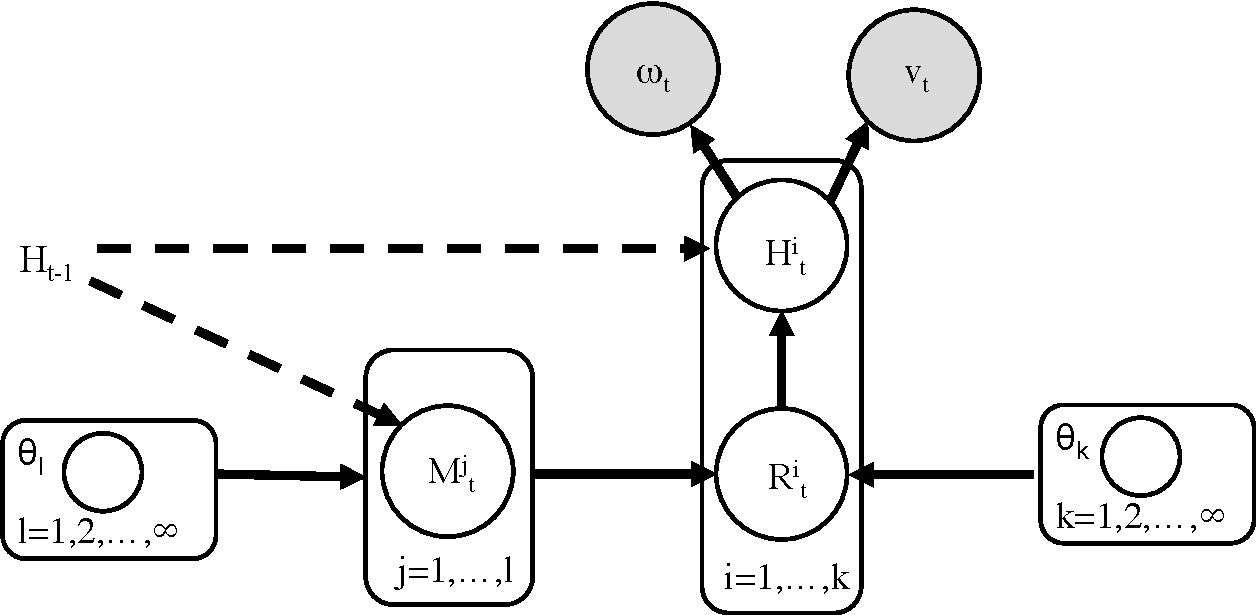
\includegraphics[width=\columnwidth]{figures/probabilistic_graphical_model.pdf}
\caption{We model the set of demonstrations as observations from a noisy stochastic process. Here we describe the graphical model for this process. There is a latent variable $H_t$ that links kinematic (shaded) and visual observations (shaded) and the \sys framework learns a discrete parametrization of this process (unshaded). }
\label{fig:pgm}
\end{figure}

\subsection{Overview of the Algorithm}
\begin{enumerate}
\item Describe the basic algorithm to learn the model and forward reference key components.
\end{enumerate}